\section*{Architecture proposée et adaptation d’Uni-Sign}

Dans cette section, nous décrivons l’architecture adoptée pour notre système de traduction automatique de la langue des signes. Elle repose sur une adaptation de l’architecture Uni-Sign~\cite{li2025unisign}, que nous avons retravaillée dans une logique de frugalité computationnelle et de modularité expérimentale. Plus précisément, nous avons :

\begin{itemize}
    \item remplacé les vidéos RGB par des séquences de poses extraites via DWPOSE ;
    \item adopté une approche \textit{gloss-free} de bout en bout ;
    \item rendu le modèle entièrement modulaire, permettant de substituer dynamiquement le backbone texte (T5, mT5 ou autre) ;
    \item introduit un mécanisme d’augmentation des embeddings (prompt) pour contextualiser l’inférence.
\end{itemize}

\subsection*{1. Pipeline général}

Le pipeline complet de notre approche est résumé comme suit :

\begin{enumerate}
    \item \textbf{Extraction des poses} : Les vidéos d’entrée sont prétraitées pour extraire des keypoints 2D/3D via l’algorithme DWPOSE. Ces points incluent les articulations du visage, des mains et du corps, structurant l'information gestuelle essentielle à la SLT.
    \item \textbf{Encodage temporel} : Les poses sont divisées en sous-séquences (\textit{sub-poses}) et encodées via un module temporel basé sur un Transformer, capturant les dépendances longues dans le temps.
    \item \textbf{Projection multimodale (optionnelle)} : L’architecture originale inclut un module de fusion guidée par les scores (PGF). Dans notre cas, ce module est désactivé pour se concentrer uniquement sur les poses.
    \item \textbf{Backbone texte modulaire} : Le décodeur de texte est défini dynamiquement dans la configuration via une classe héritée de \texttt{BaseTransformerBackbone}. Cette structure permet de tester différents backbones tels que \texttt{mT5}, \texttt{T5-v1.1}, ou nos propres variantes légères.
    \item \textbf{Augmentation des embeddings} : Un prompt fixe ou appris est inséré en tête des embeddings pour encadrer la génération, facilitant l’injection de contexte linguistique ou thématique.
\end{enumerate}

\subsection*{2. Adaptations clés}

\paragraph{Passage en \textit{pose-only}}

L’un des éléments majeurs de notre contribution est d’avoir éliminé complètement les vidéos RGB dans la phase d’entraînement comme d’inférence. Cela permet :
\begin{itemize}
    \item de réduire drastiquement les besoins en mémoire et en calcul (x5 à x10 selon les expériences) ;
    \item d’aligner le système avec les exigences de confidentialité (absence de données biométriques faciales) ;
    \item d’étudier l’hypothèse que les poses suffisent à elles seules à capturer la sémantique gestuelle.
\end{itemize}

\paragraph{Backbone Transformer généralisable}

Nous avons encapsulé toute la logique Transformer dans une classe \texttt{BaseTransformerBackbone}, fournissant les méthodes :
\texttt{forward}, \texttt{compute\_loss}, \texttt{tokenize\_labels}, etc. Ce design facilite :
\begin{itemize}
    \item la substitution rapide du backbone textuel par un autre modèle (T5, mT5, Bart...) ;
    \item l’implémentation de variantes plus légères ou spécialisées pour la tâche ;
    \item une meilleure reproductibilité du système dans d’autres langues (en changeant simplement la configuration).
\end{itemize}

\paragraph{Prompt learning et contrôle de génération}

Enfin, un vecteur prompt est introduit au niveau de l’espace des embeddings afin de guider la génération. Cette approche vise à intégrer du contexte ou de la structure grammaticale dès l’entrée dans le modèle de décodage, notamment utile pour des séquences pose-only où l’ambiguïté sémantique peut être élevée.

\subsection*{3. Visualisation et performances qualitatives}

Nos expériences montrent que, même en configuration pose-only, le modèle est capable de générer des textes informatifs, parfois différents dans la forme mais proches en sens (voir figure~\ref{fig:prediction_example}). Cela confirme que le signal gestuel est suffisant pour transmettre l’information sémantique dans la majorité des cas.

\begin{figure}[h]
    \centering
    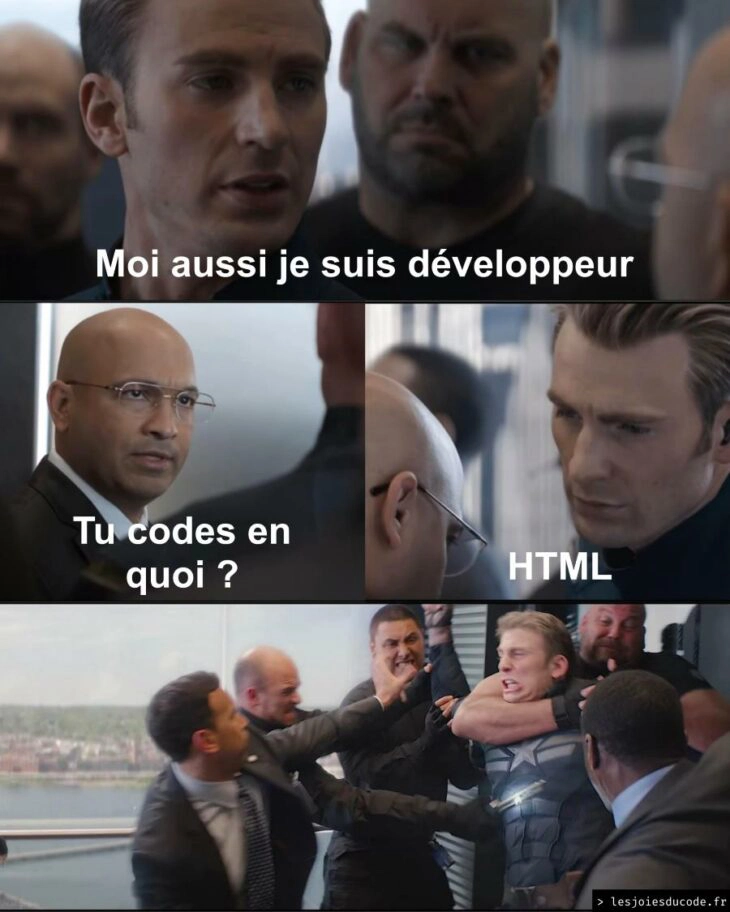
\includegraphics[width=0.45\textwidth]{figures/dev_joke.png}
    \caption{Comparaison des prédictions RGB+Pose, Pose-only, et Pose-only (Stage 1). Le modèle est capable de générer des variantes grammaticales correctes malgré la réduction du signal.}
    \label{fig:prediction_example}
\end{figure}

\subsection*{Conclusion de l’architecture}

L’architecture proposée constitue une adaptation légère, modulaire et éthique de l’approche Uni-Sign. Elle répond à des contraintes réelles de déploiement (frugalité, accessibilité, confidentialité), tout en offrant un cadre rigoureux d’expérimentation scientifique sur la valeur informationnelle des seules poses.

